Our system-design of many highly decentralized clients all pushing data
continuously to a central server means, that this server must both high
performance, high uptimes as well as the a flexible storage to ensure that it is
always possible to add more space if so needed. To ensure these properties of
the system, we have deliberately chosen a system as simple as possible to avoid
unnecessary complications, and to ensure that this central component can be
easily managed by the professional IT-staff of the department. It is
important to realized that even though it typically is not a problem if a
single client machine somewhere in the system is temporarily down (this can
happen for many reasons in a experimental lab), it is crucial that this
particular server is handled like a real production server.

To keep the server-side of things simple, we use a relational database, in our
case MySQL\cite{mysql} which is open source and provides extremely good
performance. This MySQL server contains the entire set of data of all
experimental setups, thus it is extremely easy to backup everything by simply
doing a dump of the database with regular intervals.

Since the database is only exposed to the local network, security is not a
real concern, however to protect against accidential pollution of the
various setups with irrelevant data when code is exchanged between setups, each
client has its own user name and password which is not part of the code
(typically it will be managed in ODBC-settings). In this way, code can flow back
and forth between setup without the risk of one setup accidentally logging data
to other setups tables.

\subsection{SQL}
The flexible nature of SQL allows one to extract data in many ways. Of course
complete data-sets can be retrieved by simple statements, such as 
``select {*} from table\_name``

 This data can the be handled using what ever programming
environment is comfortable for users and be used for instance to do automatic
reporting, data treatment or as input to scripts that will produce
illustrations based on the data. But SQL also allows for very efficient data-
treatment directly from the SQL-server, which can be very useful to get a
quick overview of data. As an example, this SQL-statement will directly plot
the pressure in a vacuum-chamber at 1A.M. in the morning for the last month, a
useful tool to monitor the general health of the chamber, i.e. if leaks has
developed or a valve is failing:

select unix\_timestamp(date(time)), avg(pressure) from pressure\_microreactor
where hour(time) = 1 and minute(time) between 00 and 20 and time between
``\{from\}`` and ``\{to\}`` group by date(time) order by time desc limit 30

where \{from\}  and \{to\} should be replaced with the relevant time interval.

The output from as a statement like this is illustrated in
Figure~\ref{fig:morning_pressure}. 

\begin{figure}
 \begin{center}
 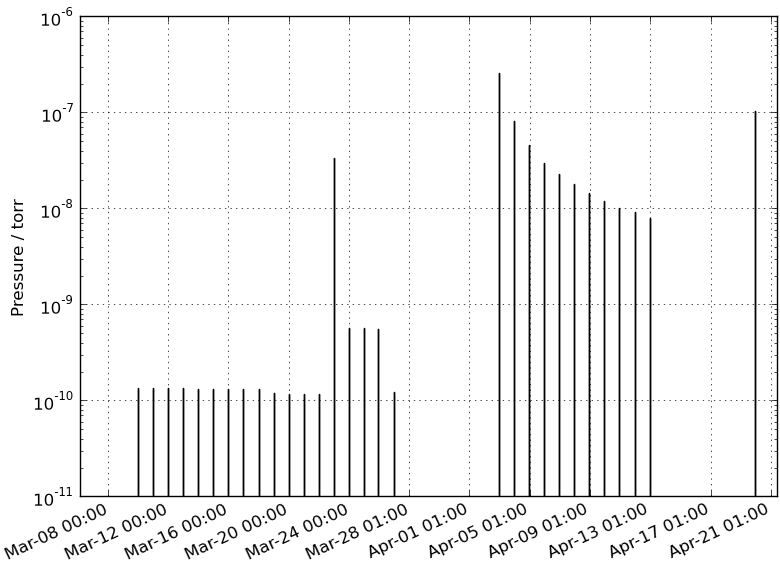
\includegraphics[width=10cm]{morning_pressure.png}
 \caption{ The morning pressure in a vacuum chamber at the department. The
   pressure gauge is unable to read high pressures, and thus no data is
   available from periods where the chamber is vented for maintenance.
   \label{fig:morning_pressure}
 } 
 \end{center}
\end{figure}

A further advantage with SQL-servers is, that SQL is reasonably standardized
and it is thus rather easy to change the choice of implementation if this for
some reason turns out to be wanted.  Several open source implementations of
SQL-servers exists.



